\DeclareOption*{\PassOptionsToClass{\CurrentOption}{abntex2}}
\ProcessOptions

\documentclass[
  % -- opções da classe memoir --
  12pt,				% tamanho da fonte
  openright,			% capítulos começam em pág ímpar (insere página vazia caso preciso)
  oneside,			% para impressão em verso e anverso. Oposto a oneside
  a4paper,			% tamanho do papel.
  % -- opções da classe abntex2 --
  %chapter=TITLE,		% títulos de capítulos convertidos em letras maiúsculas
  %section=TITLE,		% títulos de seções convertidos em letras maiúsculas
  %subsection=TITLE,	% títulos de subseções convertidos em letras maiúsculas
  %subsubsection=TITLE,% títulos de subsubseções convertidos em letras maiúsculas
  % -- opções do pacote babel --
  english,			% idioma adicional para hifenização
  french,				% idioma adicional para hifenização
  spanish,			% idioma adicional para hifenização
  brazil				% o último idioma é o principal do documento
  ]{abntex2}

\usepackage{setspace}
\usepackage{conf-ifsc}
\usepackage{hyperref}
\usepackage{graphicx}
\usepackage{caption}
\usepackage{subcaption}
\usepackage[utf8]{inputenc}
\usepackage{listings}
\usepackage{xcolor}
\usepackage{trivfloat}
\trivfloat{quadro}
\usepackage{enumitem}
\usepackage{xcolor}
\usepackage{multicol}
\usepackage{multirow}
\usepackage{hyperref}
\usepackage{float}
\floatstyle{plaintop}
\restylefloat{quadro}
\usepackage{chngcntr}
\usepackage{lipsum}
\usepackage{tocloft}
\usepackage{tocvsec2}
\usepackage{boxhandler}
\usepackage{caption}
\usepackage[font={bf,small},labelfont=small]{caption}

\usepackage{caption}
\DeclareCaptionFont{white}{\color{white}}
\DeclareCaptionFormat{listing}{\colorbox{white}{\parbox{\textwidth}{#3}}}
\captionsetup[lstlisting]{format=listing,labelfont=white,textfont=white}

\DeclareCaptionType{Codigo}[Código][Lista de Códigos]



\newcommand{\source}[1]{\caption*{\normalfont Fonte: {#1}}}


\counterwithout{equation}{chapter}
\counterwithout{figure}{chapter}
\counterwithout{table}{chapter}
\counterwithout{Codigo}{chapter}

\newcommand\ChangeRT[1]{\noalign{\hrule height #1}}


\definecolor{codegreen}{rgb}{0,0.6,0}
\definecolor{codegray}{rgb}{0.5,0.5,0.5}
\definecolor{codepurple}{rgb}{0.58,0,0.82}
\definecolor{backcolour}{rgb}{0.95,0.95,0.92}

\lstdefinestyle{mystyle}{
    backgroundcolor=\color{backcolour},
    commentstyle=\color{codegreen},
    keywordstyle=\color{magenta},
    numberstyle=\tiny\color{codegray},
    stringstyle=\color{codepurple},
    basicstyle=\ttfamily\footnotesize,
    breakatwhitespace=false,
    breaklines=true,
    captionpos=b,
    keepspaces=true,
    numbers=left,
    numbersep=5pt,
    showspaces=false,
    showstringspaces=false,
    showtabs=false,
    tabsize=2
}

\lstset{style=mystyle}

%---------------------------------------------------------------------%
%---------------------------------------------------------------------%
% PARA INCLUIR CÓDIGOS DE PROGRAMAS
%---------------------------------------------------------------------%
%---------------------------------------------------------------------%

\definecolor{dkgreen}{rgb}{0,0.6,0}
\definecolor{gray}{rgb}{0.5,0.5,0.5}
\definecolor{mauve}{rgb}{0.58,0,0.82}

\lstset{frame=tb,
  aboveskip=3mm,
  belowskip=3mm,
  showstringspaces=false,
  columns=flexible,
  numbers=left,
  numberstyle=\tiny\color{gray},
  keywordstyle=\color{blue},
  commentstyle=\color{dkgreen},
  stringstyle=\color{mauve},
  basicstyle=\ttfamily\footnotesize,
  language=C
}




%---------------------------------------------------------------------%
%---------------------------------------------------------------------%
% Informações de dados para CAPA e FOLHA DE ROSTO
%---------------------------------------------------------------------%
%---------------------------------------------------------------------%

\titulo{TÍTULO DO TRABALHO: e subtítulo se houver}

\autor{NOME DO AUTOR}

\local{FLORIANÓPOLIS}

\data{20XX.}

\orientador[Orientador:\\]{Nome do professor, titulação}


%\coorientador[Coorientador:\\]{Nome do coorientador}

\tipotrabalho{Monografia (Graduação)}

% O preambulo deve conter o tipo do trabalho, o objetivo, o nome da instituição e a área de concentração
\preambulo{Trabalho de Conclusão de Curso /  Monografia / Dissertação submetido ao Instituto Federal de Educação, Ciência e Tecnologia de Santa Catarina como parte dos requisitos para obtenção do título de Engenheiro/Tecnólogo/Especialista/Mestre em xxx.}

% \textoaprovacao{Este Trabalho foi julgado adequado para obtenção do Título de Engenheira Eletrônica em abril de 2021 e aprovado na sua forma final pela banca examinadora do Curso de Engenharia Eletrônica do instituto Federal de Educação Ciência, e Tecnologia de Santa Catarina.}

% ----------------------------------------------------------
% Configurações de aparência do PDF final
% ----------------------------------------------------------
\definecolor{blue}{RGB}{41,5,195}   % alterando o aspecto da cor azul

% ----------------------------------------------------------------------------------------
% Setup da metadata do PDF
% ----------------------------------------------------------------------------------------

\makeatletter

\hypersetup{                        % informações do PDF
  %	pagebackref=true,
  pdftitle={\@title},
  pdfauthor={\@author},
  pdfsubject={\imprimirpreambulo},
  pdfkeywords={Tag1}; {Tag2}; {Tag3}; {Tag4}; {Tag4},
  colorlinks=true,            % false: boxed links; true: colored links
  linkcolor=black,            % color of internal links
  citecolor=black,                % color of links to bibliography
  filecolor=black,            % color of file links
  urlcolor=darkgray,
  bookmarksdepth=4
}
\makeatother


%---------------------------------------------------------------------%
% Início do documento
%---------------------------------------------------------------------%

\begin{document}



\selectlanguage{brazil}
\frenchspacing


% ----------------------------------------------------------
% ELEMENTOS PRÉ-TEXTUAIS
% ----------------------------------------------------------
% \pretextual

\imprimircapa
\imprimirfolhaderosto* %(o * indica que haverá a ficha bibliográfica)

%---------------------------------------------------------------------%
% ATENÇÃO - Pergunte para a Biblioteca do IFSC
% Inserir a ficha bibliografica -
%
% Para gerar a ficha catalográfica acesse:
% http://ficha.florianopolis.ifsc.edu.br/
% Precisa ser feito pelo navegador Mozilla Firefox
%---------------------------------------------------------------------%

\imprimirficha{pdf/fichacatalografica.pdf}
%\cleardoublepage

%---------------------------------------------------------------------%
% Inserir folha de aprovação
%---------------------------------------------------------------------%


%\imprimiraprovacao
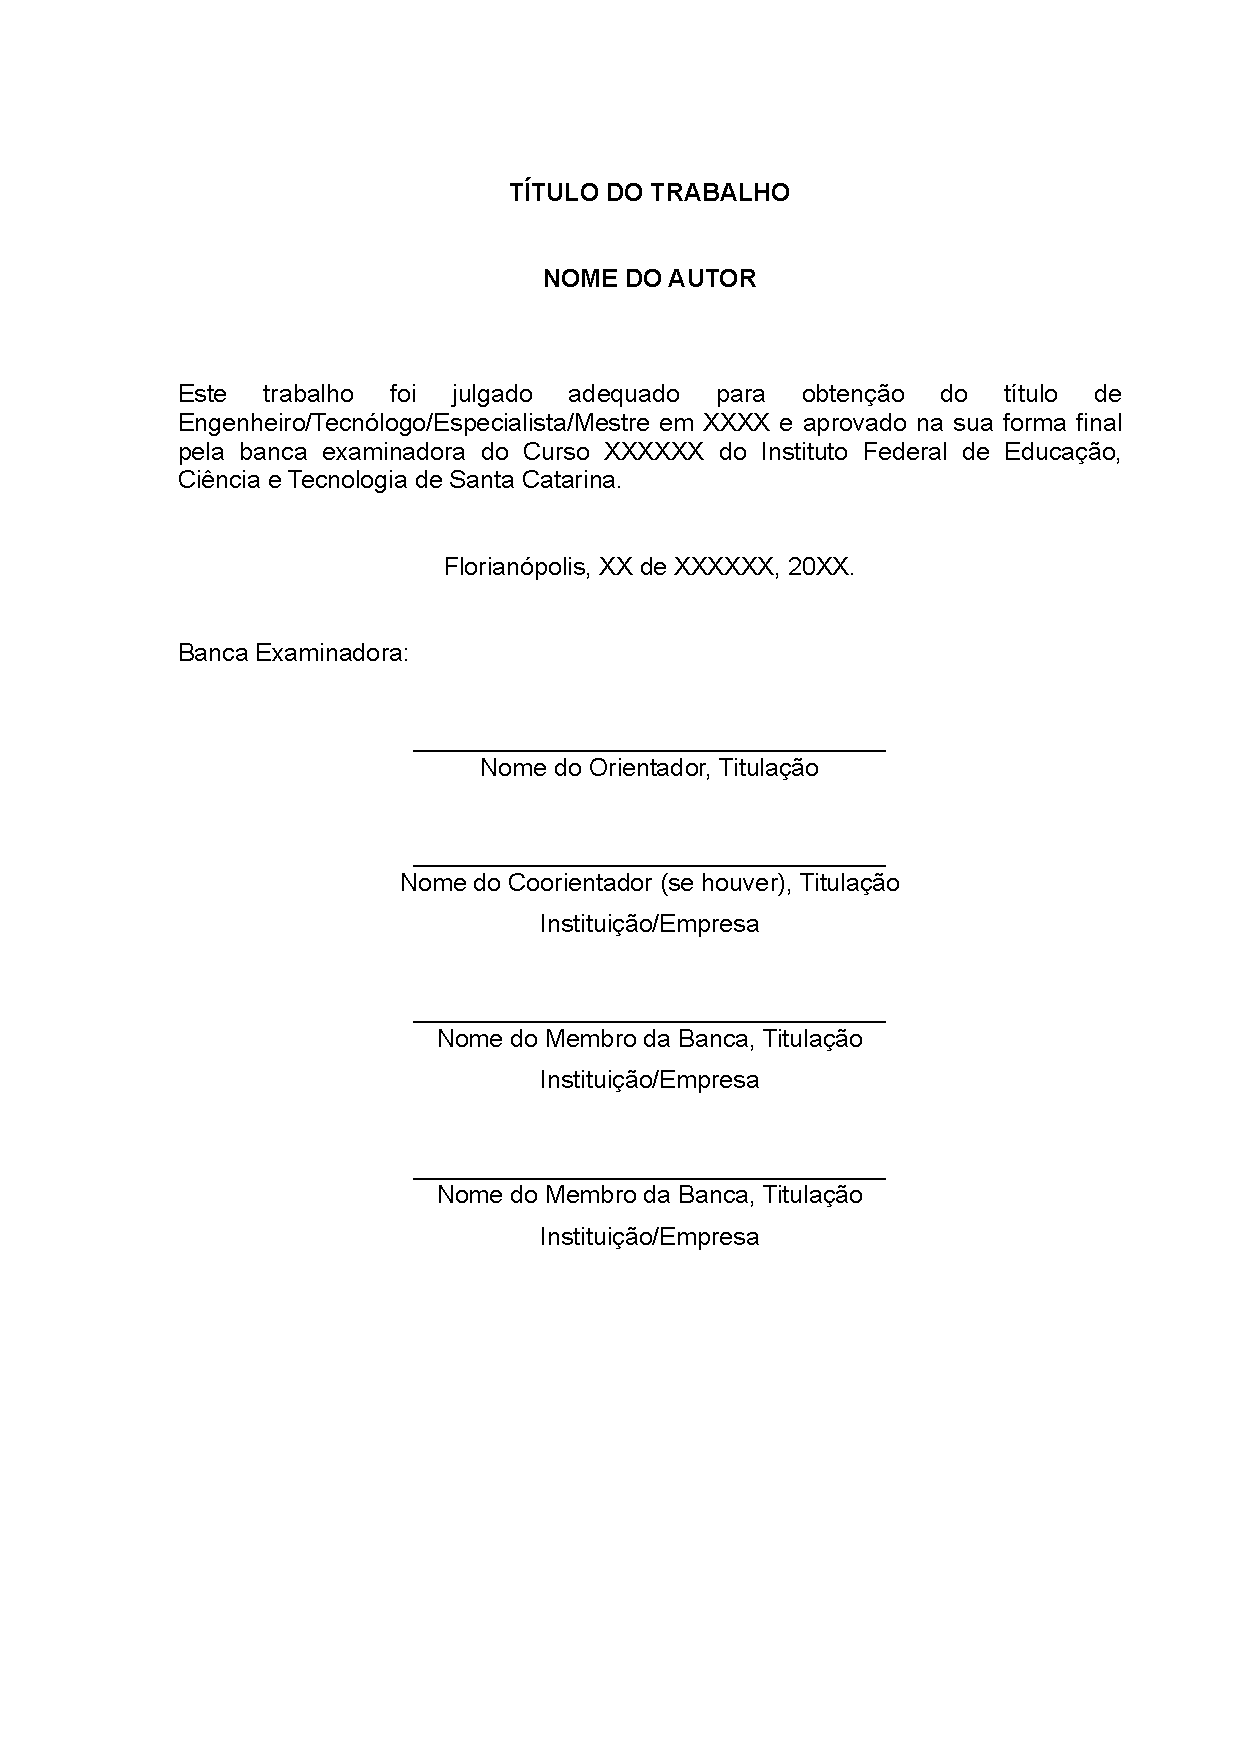
\includepdf[pages=-]{pdf/tcc-aprovado.pdf}

%\cleardoublepage

%---------------------------------------------------------------------%
% Dedicatória
%---------------------------------------------------------------------%
\begin{dedicatoria}
    \vspace*{\fill}
  \begin{flushright}
        (Dedicatória é um elemento opcional.\\
            Texto alinhado no canto inferior direito.\\
            Não deve ultrapassar uma página.)
  \end{flushright}
\end{dedicatoria}




%---------------------------------------------------------------------%
% Agradecimentos
%---------------------------------------------------------------------%
\begin{agradecimentos}
    Elemento opcional que não pode ultrapassar o limite de uma página.
\end{agradecimentos}
% ---

%---------------------------------------------------------------------%
% Epígrafe
%---------------------------------------------------------------------%
\begin{epigrafe}
    \vspace*{\fill}
  \begin{flushright}
        (Epígrafe é um elemento opcional.\\
        Texto alinhado no canto inferior direito.\\
            Não deve ultrapassar uma página.)
  \end{flushright}
\end{epigrafe}

%---------------------------------------------------------------------%
% RESUMOS
%---------------------------------------------------------------------%
% resumo em português
\setlength{\absparsep}{18pt} % ajusta o espaçamento dos parágrafos do resumo
\renewcommand{\baselinestretch}{1}
\begin{resumo}
    O resumo deve mostrar a natureza e o objetivo do trabalho, o método que foi empregado, os resultados e as conclusões. O resumo deve conter entre 150 e 500 palavras e constitui-se de um único parágrafo, sem recuo.


   \noindent
    \textbf{Palavras-chave}: Primeira palavra-chave. Segunda palavra-chave. Terceira palavra-chave. Quarta palavra-chave (opcional). Quinta palavra-chave (opcional).
\end{resumo}

% resumo em inglês
\renewcommand{\baselinestretch}{1}
\begin{resumo}[Abstract]
 \begin{otherlanguage*}{english}

   The abstract should show the nature and scope of work, the method that was used, the results and conclusions. The abstract may contain between 150 and 500 words, and it must be only one paragraph.


   %\vspace{-0.8cm}

   \noindent
   \textbf{Keywords}: First keyword. Second keyword. Third keyword. Fourth keyword (optional). Fifth keyword (optional).
 \end{otherlanguage*}
\end{resumo}


%---------------------------------------------------------------------%
% inserir lista de ilustrações
%---------------------------------------------------------------------%
\renewcommand{\listfigurename}{Lista de Figuras}
\pdfbookmark[0]{\listfigurename}{lof}
\listoffigures*
\cleardoublepage

%---------------------------------------------------------------------%
% inserir lista de quadros
%---------------------------------------------------------------------%

\renewcommand{\listquadroname}{Lista de quadros}
\newfloat{quadro}{\quadroname}{loq}[chapter]
\setfloatlocations{quadro}{hbtp}
\newlistof{listofquadros}{loq}{\listquadroname}
\newlistentry{quadro}{loq}{0}
\renewcommand{\cftquadroname}{\quadroname\space}
\renewcommand*{\cftquadroaftersnum}{\hfill\textendash\hfill}
\counterwithout{quadro}{chapter}
\listofquadros*
\cleardoublepage



%---------------------------------------------------------------------%
% inserir lista de tabelas
%---------------------------------------------------------------------%
\pdfbookmark[0]{\listtablename}{lot}
\listoftables*
\cleardoublepage



%---------------------------------------------------------------------%
% inserir lista de Codigos
%---------------------------------------------------------------------%


\renewcommand{\listCodigoname}{Lista de Códigos}
\setfloatlocations{Codigo}{hbtp}
\newlistof{listofCodigos}{loc}{\listCodigoname}
\newlistentry{Codigo}{loc}{0}
\renewcommand{\cftCodigoname}{\Codigoname\space}
\renewcommand*{\cftCodigoaftersnum}{\hfill\textendash\hfill}
\counterwithout{Codigo}{chapter}
\newfloat{Codigo}{\Codigoname}{loc}[chapter]
\listofCodigos*
\cleardoublepage









%---------------------------------------------------------------------%
% inserir lista de listings
%---------------------------------------------------------------------%
%\pdfbookmark[0]{\lstlistlistingname}{lol}
%\listoflistings
%\cleardoublepage

%---------------------------------------------------------------------%
% inserir lista de abreviaturas e simbolos
%---------------------------------------------------------------------%
%\listofabrev{tex/00-Abreviaturas}
\imprimirlistadeabreviaturas

% \imprimirlistadesimbolos
\cleardoublepage

%---------------------------------------------------------------------%
% inserir o sumario

%---------------------------------------------------------------------%


\setlength{\cftbeforechapterskip}{4pt plus 0pt}
\pdfbookmark[0]{\contentsname}{toc}
\tableofcontents*
\cleardoublepage




% ----------------------------------------------------------
% ELEMENTOS TEXTUAIS
% ----------------------------------------------------------
\textual

% ----------------------------------------------------------
% Inclusão dos capítulos que estão em outros arquivos .tex
% ----------------------------------------------------------

\chapter{Introdução}


Texto texto texto texto texto texto texto texto texto texto texto texto texto texto texto texto texto texto texto texto texto texto texto texto texto texto texto texto texto texto texto texto texto texto texto texto texto texto texto. \abreviatura{IFSC}{Instituto Federal de Santa Catarina}
\abreviatura{LER}{Lesão por Esforço Repetitivo} 
\abreviatura{IoT}{\textit{Internet of Things} (Internet das Coisas)}
\abreviatura{ANEEL}{Agência Nacional de Energia Elétrica}
\abreviatura{IBM}{\textit{International Business Machines}}


\section{Justificativa}

Texto texto texto texto texto texto texto texto texto texto texto texto texto texto texto texto texto texto texto texto texto texto texto texto texto texto texto texto texto texto texto texto texto texto texto texto texto texto texto.

\section{Definição do Problema}

Texto texto texto texto texto texto texto texto texto texto texto texto texto texto texto texto texto texto texto texto texto texto texto texto texto texto texto texto texto texto texto texto texto texto texto texto texto texto texto \cite{ref:vazquez}.

\section{Objetivo Geral}

Texto texto texto texto texto texto texto texto texto texto texto texto texto texto texto texto texto texto texto texto texto texto texto texto texto texto texto texto texto texto texto texto texto texto texto texto texto texto texto.

\section{Objetivos Específicos}

Texto texto texto texto:
\begin{alineas}
    \item texto texto texto texto texto texto texto texto texto texto texto texto texto texto texto texto texto texto texto texto texto texto texto texto texto texto texto texto texto texto texto texto texto texto texto texto texto texto;
    \item texto texto texto texto texto texto texto texto texto texto texto texto texto texto texto texto texto texto texto texto texto texto texto texto texto texto texto texto texto texto texto texto texto texto texto texto texto texto; 
    \item texto texto texto texto texto texto texto texto texto texto texto texto texto texto texto texto texto texto texto texto texto texto texto texto texto texto texto texto texto texto texto texto texto texto texto texto texto texto.
\end{alineas}
    
\section{Estrutura do Trabalho}

Texto texto texto texto texto texto texto texto texto texto texto texto texto texto texto texto texto texto texto texto texto texto. 

\chapter{Fundamentação Teórica}

Texto texto texto texto texto texto texto texto texto texto texto texto texto texto texto texto texto texto texto texto texto texto texto texto texto texto texto texto texto texto texto texto texto texto texto texto texto texto texto.

\section{Subtítulo Secundário 1}

Texto texto texto texto texto texto texto texto texto texto texto texto texto texto texto texto texto texto texto texto texto texto texto texto texto texto texto texto texto texto texto texto texto texto texto texto texto texto texto, como mostra o Quadro \ref{quadro1}.


\begin{quadro}[h]
\centering

\caption{Tipos de energia analisados}
\begin{tabular}{|c|c|}
\hline
\textbf{Ano} & \textbf{Tipos de energia} \\ \hline
2017         & Mecânica                  \\ \hline
2018         & Térmica                   \\ \hline
2019         & Elétrica                  \\ \hline
2020         & Química                   \\ \hline
2021         & Atômica                   \\ \hline
\end{tabular}
\label{quadro1}
\\
\small{Fonte: Elaboração própria (2021).} 
\end{quadro}

\section{Subtítulo Secundário 2}

As citações diretas com menos de três linhas “devem estar entre aspas e devem mostrar entre parênteses o ano e a página da obra consultada.” (AUTOR, ano, página). Já as citações com mais de três linhas devem ser recuadas da margem esquerda em 4 cm, tamanho da fonte 10, espaçamento simples e texto sem aspas (ABNT, 2002, p. 2).



 \begin{citacao}
            \begin{alineas}[leftmargin=\leftskip+\labelwidth-\labelsep]
                Texto texto texto texto texto texto texto texto. Texto texto texto texto texto texto. Texto texto texto texto texto texto texto texto texto. Texto texto texto texto texto texto Texto texto texto texto texto texto. Texto texto texto texto texto texto. (\citeauthor{ref:ibmm}, \citeyear{ref:ibmm}, p. 20).
            \end{alineas}
\end{citacao}



\subsection{Subtítulo Terciário}

Texto texto texto texto texto texto texto texto texto texto texto texto texto texto texto texto texto texto texto texto texto texto texto texto texto texto texto texto texto texto texto texto texto.


\subsubsection{Subtítulo Quaternário}

Texto texto texto texto texto texto texto texto texto texto texto texto texto texto texto texto texto texto texto texto texto texto texto texto texto texto texto texto texto texto texto texto texto  (conforme exposto na Figura \ref{fig:motor}).



    \begin{figure}[H]
    	\centering
    	\caption{Motor Weg W22}
    	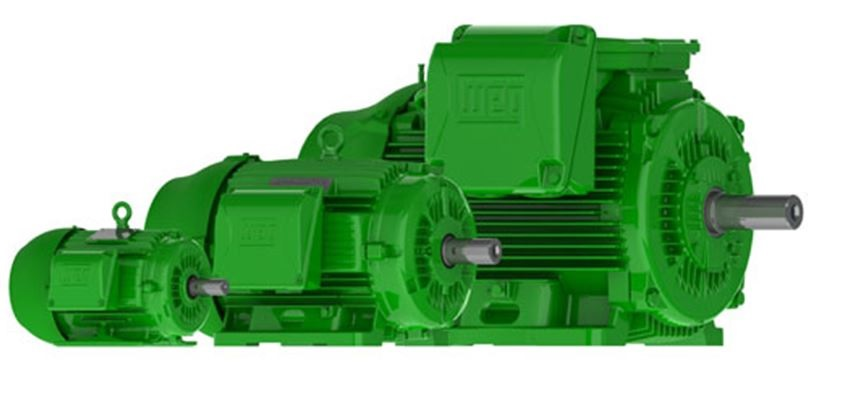
\includegraphics[scale=0.45]{figuras/motor.jpg}
    	\label{fig:motor}
    	\\
        \vspace{-0.8cm}\hspace{-7cm}\small{Fonte: WEG (2014).} 
    \end{figure}
    
    Texto texto texto texto texto texto texto texto texto texto texto texto texto texto texto conforme indica a Tabela \ref{tabela1}.

    

\begin{table}[h]
\centering
\caption{Produção de petróleo na Bahia}
\begin{tabular}{ c c }
\ChangeRT{2pt}
Ano  & Produção (1000 t) \\ \ChangeRT{2pt}
1996 & 2.536             \\ 
1997 & 2.665             \\ 
1998 & 3.056             \\ 
1999 & 3.567             \\ 
2021 & Atômica           \\ \ChangeRT{2pt}
\end{tabular}
\label{tabela1}
\\
\small{Fonte: Adaptado de ANP (2000).} 
\end{table}



    
    Texto texto texto texto texto texto texto texto texto texto texto texto texto texto texto texto texto texto texto texto texto texto texto texto texto texto texto texto texto texto texto texto texto 
    Texto texto texto texto texto texto texto texto texto texto texto texto texto texto texto texto texto texto texto texto texto texto texto texto texto texto texto texto texto texto texto texto texto como evidencia a Figura  \ref{fig:diagrama}.
    
    
    
    \begin{figure}[H]
    	\centering
    	\caption{Diagrama Fasorial}
    	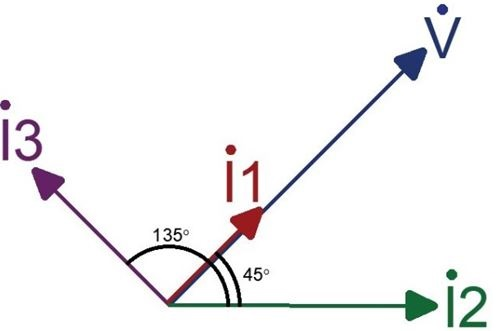
\includegraphics[scale=0.45]{figuras/diagrama.jpg}
    	\label{fig:diagrama}
    	\\
    	\vspace{0.2cm}\hspace{-3cm}\small{Fonte: Silva (2020).}
    \end{figure}
    
    Texto texto texto texto texto texto texto texto texto texto texto texto texto texto texto texto texto texto texto texto texto texto texto texto texto texto texto texto texto texto texto texto, conforme mostra a Equação \ref{eq:baskara}.
    
\begin{equation} \label{eq:baskara}
  x=\frac{-b\pm\sqrt{b^2-4ac}}{2a}
\end{equation} 

\chapter{Metodologia}

Texto texto texto texto texto texto texto texto texto texto texto texto texto texto texto texto texto texto texto texto texto texto texto texto texto texto texto texto texto texto texto texto texto texto texto texto texto texto texto \cite{ref:Nuseibeh}.

\section{Métodos Aplicados}

Texto texto texto texto texto texto texto texto texto texto texto texto texto texto texto texto texto texto texto texto texto texto texto texto texto texto texto texto texto texto texto texto texto texto texto texto texto texto texto.

\chapter{Apresentação dos Resultados}

Texto texto texto texto texto texto texto texto texto texto texto texto texto texto texto texto texto texto texto texto texto texto texto texto texto texto texto texto texto texto texto texto texto texto texto texto texto texto texto.

\section{Análise e discussão dos resultados}

Texto texto texto texto texto texto texto texto texto texto texto texto texto texto texto texto texto texto texto texto texto texto texto texto texto texto texto texto texto texto texto texto texto texto texto texto texto texto texto.

Os  códigos \ref{programa1} e \ref{programa2} apresentam o exemplo de um código escrito na linguagem de programação C.  

\begin{Codigo}[h]
\lstinputlisting[firstline=1, lastline=6]{codigos/exemplo.c}
\caption{Exemplo de Código escrito em C}
\label{programa1}
\end{Codigo}

Texto texto texto texto texto texto texto texto texto texto texto texto texto texto texto texto texto texto texto texto texto texto texto texto texto texto texto texto texto texto texto texto texto texto texto texto texto texto texto. O firstnumber=auto reinicia a numeração das linhas em 1.


\begin{Codigo}[h]
\lstinputlisting[firstnumber=auto, firstline=1, lastline=6]{codigos/exemplo.c}
\caption{Mesmo Exemplo de Código escrito em C}
\label{programa2}
\end{Codigo}

\chapter{Considerações Finais}

Texto texto texto texto texto texto texto texto texto texto texto texto texto texto texto texto texto texto texto texto texto texto texto texto texto texto texto texto texto texto texto texto texto texto texto texto texto texto texto.

\section{Sugestões para trabalhos futuros}

Texto texto texto texto texto texto texto texto texto texto texto texto texto texto texto texto texto texto texto texto texto texto texto texto texto texto texto texto texto texto texto texto texto texto texto texto texto texto texto.




% ----------------------------------------------------------
% ELEMENTOS PÓS-TEXTUAIS
% ----------------------------------------------------------
\postextual
% ----------------------------------------------------------

% ----------------------------------------------------------
% Referências bibliográficas
% ----------------------------------------------------------
\bibliography{referencias}

% ----------------------------------------------------------
% Apêndices
% ----------------------------------------------------------
 \begin{apendicesenv}
     \partapendices
     \chapter{Título}

\chapter{Título}
 \end{apendicesenv}

% ----------------------------------------------------------
% Anexos
% ----------------------------------------------------------
 \begin{anexosenv}
     \partanexos
     \chapter{Título}

\chapter{Título}
 \end{anexosenv}

%---------------------------------------------------------------------
% INDICE REMISSIVO
%---------------------------------------------------------------------
%\phantompart
%\printindex
%---------------------------------------------------------------------

\end{document}
